% This is "sig-alternate.tex" V1.9 April 2009
% This file should be compiled with V2.4 of "sig-alternate.cls" April 2009
%
% This example file demonstrates the use of the 'sig-alternate.cls'
% V2.4 LaTeX2e document class file. It is for those submitting
% articles to ACM Conference Proceedings WHO DO NOT WISH TO
% STRICTLY ADHERE TO THE SIGS (PUBS-BOARD-ENDORSED) STYLE.
% The 'sig-alternate.cls' file will produce a similar-looking,
% albeit, 'tighter' paper resulting in, invariably, fewer pages.
%
% ----------------------------------------------------------------------------------------------------------------
% This .tex file (and associated .cls V2.4) produces:
%       1) The Permission Statement
%       2) The Conference (location) Info information
%       3) The Copyright Line with ACM data
%       4) NO page numbers
%
% as against the acm_proc_article-sp.cls file which
% DOES NOT produce 1) thru' 3) above.
%
% Using 'sig-alternate.cls' you have control, however, from within
% the source .tex file, over both the CopyrightYear
% (defaulted to 200X) and the ACM Copyright Data
% (defaulted to X-XXXXX-XX-X/XX/XX).
% e.g.
% \CopyrightYear{2007} will cause 2007 to appear in the copyright line.
% \crdata{0-12345-67-8/90/12} will cause 0-12345-67-8/90/12 to appear in the copyright line.
%
% ---------------------------------------------------------------------------------------------------------------
% This .tex source is an example which *does* use
% the .bib file (from which the .bbl file % is produced).
% REMEMBER HOWEVER: After having produced the .bbl file,
% and prior to final submission, you *NEED* to 'insert'
% your .bbl file into your source .tex file so as to provide
% ONE 'self-contained' source file.
%
% ================= IF YOU HAVE QUESTIONS =======================
% Questions regarding the SIGS styles, SIGS policies and
% procedures, Conferences etc. should be sent to
% Adrienne Griscti (griscti@acm.org)
%
% Technical questions _only_ to
% Gerald Murray (murray@hq.acm.org)
% ===============================================================
%
% For tracking purposes - this is V1.9 - April 2009

\documentclass{sig-alternate}
\usepackage{verbatim}
\usepackage{url}

\begin{document}
%
% --- Author Metadata here ---
\conferenceinfo{I-SEMANTICS Triplification Challenge}{2010 Graz, Austria}
%\CopyrightYear{2007} % Allows default copyright year (20XX) to be over-ridden - IF NEED BE.
%\crdata{0-12345-67-8/90/01}  % Allows default copyright data (0-89791-88-6/97/05) to be over-ridden - IF NEED BE.
% --- End of Author Metadata ---

\title{VMLD}
%%
%\title{Application name or something\titlenote{(Produces the permission block, and
%copyright information). For use with
%SIG-ALTERNATE.CLS. Supported by ACM.}}
%%
%\subtitle{[Some subtitle Triplification Challenge]
%\titlenote{A full version of this paper is available as
%\textit{Author's Guide to Preparing ACM SIG Proceedings Using
%\LaTeX$2_\epsilon$\ and BibTeX} at
%\texttt{www.acm.org/eaddress.htm}}}
%
% You need the command \numberofauthors to handle the 'placement
% and alignment' of the authors beneath the title.
%
% For aesthetic reasons, we recommend 'three authors at a time'
% i.e. three 'name/affiliation blocks' be placed beneath the title.
%
% NOTE: You are NOT restricted in how many 'rows' of
% "name/affiliations" may appear. We just ask that you restrict
% the number of 'columns' to three.
%
% Because of the available 'opening page real-estate'
% we ask you to refrain from putting more than six authors
% (two rows with three columns) beneath the article title.
% More than six makes the first-page appear very cluttered indeed.
%
% Use the \alignauthor commands to handle the names
% and affiliations for an 'aesthetic maximum' of six authors.
% Add names, affiliations, addresses for
% the seventh etc. author(s) as the argument for the
% \additionalauthors command.
% These 'additional authors' will be output/set for you
% without further effort on your part as the last section in
% the body of your article BEFORE References or any Appendices.

\numberofauthors{3} %  in this sample file, there are a *total*
% of EIGHT authors. SIX appear on the 'first-page' (for formatting
% reasons) and the remaining two appear in the \additionalauthors section.
%
\author{
% You can go ahead and credit any number of authors here,
% e.g. one 'row of three' or two rows (consisting of one row of three
% and a second row of one, two or three).
%
% The command \alignauthor (no curly braces needed) should
% precede each author name, affiliation/snail-mail address and
% e-mail address. Additionally, tag each line of
% affiliation/address with \affaddr, and tag the
% e-mail address with \email.
%
% 1st. author
%\titlenote{}
\alignauthor
Daniel Garijo\\
       \affaddr{OEG-DIA}\\
       \affaddr{Facultad de Inform�tica}\\
       \affaddr{Universidad Polit�cnica de Madrid}\\
       \email{dgarijo@fi.upm.es}
% 2nd. author
\alignauthor
Idafen Santana P\'erez\\
       \affaddr{OEG-DIA}\\
       \affaddr{Facultad de Inform�tica}\\
       \affaddr{Universidad Polit�cnica de Madrid}\\
       \email{isantana@fi.upm.es}
% 3rd. author
\alignauthor 
Boris Villaz\'on-Terrazas\\
       \affaddr{OEG-DIA}\\
       \affaddr{Facultad de Inform�tica}\\
       \affaddr{Universidad Polit�cnica de Madrid}\\
       \email{bvillazon@fi.upm.es}
}
% There's nothing stopping you putting the seventh, eighth, etc.
% author on the opening page (as the 'third row') but we ask,
% for aesthetic reasons that you place these 'additional authors'
% in the \additional authors block, viz.
\date{30 April 2011}
% Just remember to make sure that the TOTAL number of authors
% is the number that will appear on the first page PLUS the
% number that will appear in the \additionalauthors section.

\maketitle
\begin{abstract}
We present the process that has been followed for the development of an application that makes use of several heterogeneous datasets that are related to .....
\end{abstract}

% A category with the (minimum) three required fields
\category{H.3}{Information Storage and Retrieval}{Miscellaneous}
%A category including the fourth, optional field follows...
\category{E.2}{Data storage representations}{Linked Representations}

\terms{Design, Experimentation}

\keywords{linked data, linked government data}

\section{Introduction}\label{sec:intro}
Virtualization is a computing technology that enables a single user to access multiple physical devices. Virtualization may also be used for running multiple applications on each server rather than just one; this in turn reduces the number of servers companies need to purchase and manage. It enables to consolidate servers and do more with less hardware. In the other hand, cloud computing offers scalable infrastructure and software off site, saving labor, hardware, and power costs. Financially, the cloud’s virtual resources are typically cheaper than dedicated physical resources connected to a personal computer or network. With cloud computing, the software programs are not running from the personal computer, but rather are stored on servers housed elsewhere and accessed via the Internet. \cite{Steinder_2008}.

Linked Data principles are being adopted by an increasing number of data providers, getting as a result a global data space on the Web containing billions of RDF triples \cite{Heath_Bizer_2011}. Moreover, Linked Data technologies are being using to share data covering a wide range of different topical domains, such as Media, Geographic, Government, Publications, Cross-domain, and Life sciences. However, there are no datasets that cover the Computer Science domain, which means that we, as computer scientists, are not taking the advantages of adopting Linked Data Principles to our own domain.

This paper aims at showing that is possible to adopt Linked Data Principles within the Computer Science domain, specifically in the virtualization and cloud computing fields. In this paper, we present the process that has been followed for the development of Linked Data applications that facilitate the search and discovery of virtual machine images in a systematic way. The rest of paper is organized as follows: Section \ref{sec:ec2} introduces the Amazon Elastic Compute Cloud (EC2) AMI, Section \ref{sec:process} explains the process we followed for the generation of linked
data, Section \ref{sec:apps} describes the linked data applications that we built, and finally, Section \ref{sec:conclusions} presents the conclusions and future work.









\begin{figure*}[h!t!]
  \caption{High Level Architecture}
  \centering
    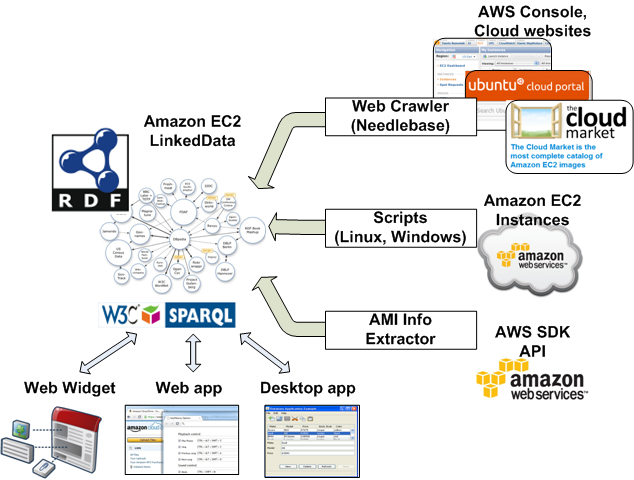
\includegraphics[scale=0.6]{EC2LD.png}
   \label{fig:architecture}
\end{figure*}

\section{Amazon EC2 AMI}\label{sec:ec2}

Nowadays the advancements of cloud computing have made it possible for us to have different environments for computing without having the need to have a dedicated infrastructure for each of the different environments we require. One of the main advantage of virtualized environment is that it is possible to recreate the same environment as many times as you want with a minimal effort. This put the computer users lives at ease because they can use a virtual machines for different temporary tasks without having the trouble to change the configuration of the personal machines. This ability can be very useful in scenarios like reproducing environments for software testing, to try out software before installing them on a physical machine i.e. as a staging machine. 

If it is possible to use already prepared virtual machines which matches the requirements, for example, the architecture, i.e., it is 32 bits or 64 bits, the operation system, storage and memory requirements it would save a lot of time and effort of people trying to prepare a computing environment for a given task. In other words, if we could facilitate the search and discovery of virtual machine images in a systematic way, we could build a lot of semantic applications on top of this that will automate this process and make the use of cloud computing for these tasks much easier. 

Amazon Elastic Compute Cloud (EC2) is a central part of Amazon.com's cloud computing platform, Amazon Web Services\footnote{\url{http://aws.amazon.com/ec2/}} (AWS). EC2 allows users to rent virtual computers on which to run their own computer applications. EC2 allows scalable deployment of applications by providing a Web service through which a user can boot an Amazon Machine Image to create a virtual machine, which Amazon calls an ``instance'', containing any software desired. A user can create, launch, and terminate server instances as needed, paying by the hour for active servers, hence the term ``elastic''. EC2 provides users with control over the geographical location of instances that allows for latency optimization and high levels of redundancy.

\section{EC2 AMI Linked Data Life Cycle}\label{sec:process}
In this section we briefly describe our process for generating, interconnecting, and publishing EC2 AMI linked data. This process was inspired by existing methodological guidelines \cite{VillazonTerrazas_2011}, which propose an iterative incremental life cycle model where EC2 AMI LD gets
continuously improved and extended.  The EC2 AMI Linked Data life cycle consists of five main activities, namely specification, modelling, generation, publication and exploitation. We focus on the description of the (1) specification of the resultant application, section \ref{sec:usecase}, and (2) data extraction and RDF transformation, sectionv\ref{sec:dataex}.

The goal is to create a LinkedData dataset about Amazon virtual machine images. Thanks to this dataset, we are able to build applications that can query the dataset using the defined ontology and help the users find Amazon Machine Images (AMI) that suit their requirements. Figure \ref{fig:architecture} shows the high level architecture.

\subsection{Use cases for AmazonMachineImage reuse}\label{sec:usecase}
Among many other advantages of cloud computing like scalability, high accessibility, and cost saving the ability to reuse a virtual machine as many times becomes a time saver in most of the cloud scenarios. Most cloud users create several master templates of the virtual machines images and use the appropriate one whenever necessary. This is far more efficient compared to setting up physical machines as the virtual machine images which are not currently executing will only consume storage space but no CPU power or memory. It is even better if one can use a public virtual machine image which satisfies the task at hand because it bring the setting up time to a bare minimum. 

There are many use cases where it is very useful to find and reuse an existing virtual machine image without spending time on preparing the environment. For example, one might want to find a virtual machine environment which has a similar characteristics to a physical machine to experiment different configurations or settings without having the risk of corrupting the own machines. It also make it possible to start things from the scratch with another instance of the same virtual image. Moreover, it is becoming common for software vendors to provide links to public virtual machine images which the users can use as a sandbox to first try the software on a virtual machine without installing on their own machines.    

\subsection{Amazon Machine Image data extraction}\label{sec:dataex}
Amazon EC2 LinkedData dataset is created by merging the data acquired by several different sources. The main source is the API provided by AWS SDK for Java \footnote{\url{http://aws.amazon.com/documentation/sdkforjava/}}. An AMI Information Extractor java application will iterate through all the public Amazon Virtual Machine images and extract the data available from the API. However, the AWS SDK lacks the ability to extract several important attributes like operating system, or the image size which are essential to make this dataset useful in real life scenarios. The challenge is overcome by extracting information from other sources and aggregating them to the dataset. There are websites and portals which provides a richer set of attributes about Amazon Machine Images which contains the aforementioned information as unstructured data available as wep pages. Examples of these sites include the AWS Management Console \footnote{http://aws.amazon.com/console/}, Ubuntu Cloud Portal \footnote{http://cloud.ubuntu.com/}, and The Cloud Market catalog {http://thecloudmarket.com/}. Needlebase platform \footnote{http://needlebase.com/} is used to acquiring, integrating, and cleansing information from these sites and feed them to the Amazon EC2 LinkedData dataset. Even more detailed information about a given AMI can be extracted by a running scripts inside the Amazon instances created using the given AMI. Two scripts for Windows and Linux are made available for Amazon users which they can run to upload additional data about an AMI.       

Finally, it is worth mentioning that the SPARL endpoint is available at \url{http://mccarthy.dia.fi.upm.es:8892/sparql}.
%\vspace{5mm}
\section{EC2LD applications}\label{sec:apps}
We have built three applications that consume the Amazon EC2 LinkedData and provide users AmazonMachineImage ids which match their requirements. These applications are a web widget, a desktop application, a web application. The web widget which is implemented as a Google Gadget \footnote{https://developers.google.com/gadgets/} can be embedded in web pages. Once configured with certain properties, this widget can communicate with the SPARQL endpoint and dynamically fetch the amazon virtual machine images which match the requirements. Figure \ref{fig:config} shows an example of the parameters. This can be a good addition to the software providers i.e. they can include this widget in the download pages so that users know in which public virtual machine images they can try this software.

\begin{figure}[h!t!]
  \caption{Configuration parameters of the web widget}
  \centering
    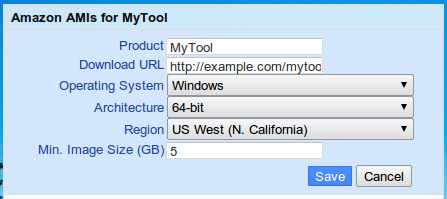
\includegraphics[width=0.5\textwidth]{gadget-config.png}
   \label{fig:config}
\end{figure}

The VMI Finder desktop application can run on a computing environment and gather the data and then will create a SPARQL query based on those information to query the SPARQL endpoint exposed by Amazon EC2 LinkedData. Users can manually modify the information that has been automatically collected before executing the query by editing, adding, or removing any information. The query result will provide a set of AmazonMachineImage ids which matches the computing environment it runs. The web application also provide a similar functionality where users can directly search for AmazonMachineImages via a web interface. Figure \ref{fig:results} depicts the search results.

\begin{figure}[h!t!]
  \caption{Search results of the web widget}
  \centering
    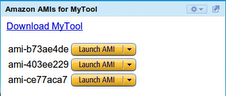
\includegraphics[scale=0.8]{gadget-results.png}
   \label{fig:results}
\end{figure}

The applications are available at \url{http://mccarthy.dia.fi.upm.es/ec2ld/}

\section{Conclusions and future work}
In this paper we have presented an application that makes use of several  ...

%ACKNOWLEDGMENTS are optional
\section{Acknowledgments}
This work has been supported by the R\&D project Webn1. We would like to kindly thanks Alexander de Le\'on and Miguel Angel Garc\'{i}a.
%
% The following two commands are all you need in the
% initial runs of your .tex file to
% produce the bibliography for the citations in your paper.
\bibliographystyle{abbrv}
\bibliography{sigproc}  % sigproc.bib is the name of the Bibliography in this case
% You must have a proper ".bib" file
%  and remember to run:
% latex bibtex latex latex
% to resolve all references
%
% ACM needs 'a single self-contained file'!
%
%APPENDICES are optional
%\balancecolumns
\end{document}
